\section{¿Que son los modelos dimensionales?} 
El modelado dimensional reside en la evidente simplicidad de los modelos y en la forma natural que la gente de negocios y la gente técnica puedan entender lo que significan estos modelos.
\\

Los modelos dimensionales tienen dos expresiones diferentes, lógica y física. La expresión puramente lógica queda plasmada en el siguiente diagrama.
\\
\\
	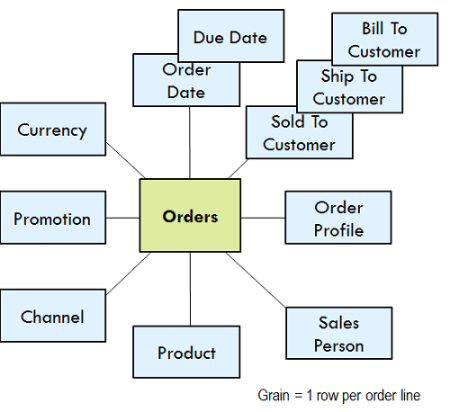
\includegraphics[width=7cm]{./Imagenes/dimensional} 

El diagrama del modelo lógico se transformará con bastante rapidez a un diseño técnico más específico repleto de nombres de tablas, nombres de campos, y declaraciones de claves primarias y foráneas.
\\
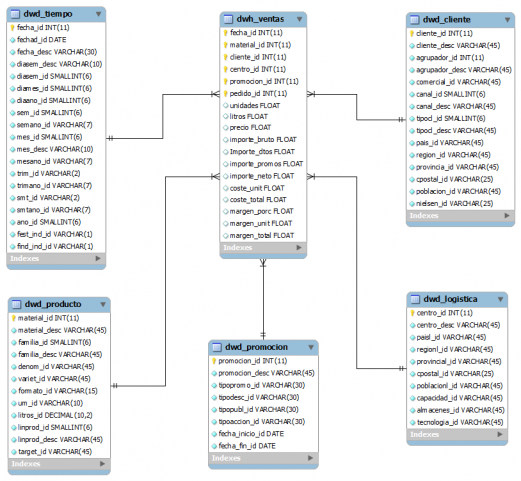
\includegraphics[width=7cm]{./Imagenes/fisica} 
\\
Recuperado de: datawarehouse.es
